\documentclass{vldb}
\usepackage{graphicx}
\usepackage{hyperref}
\usepackage{balance}  % for  \balance command ON LAST PAGE  (only there!)
\usepackage{placeins}
\usepackage{tabularx}
\usepackage[space]{grffile}



\begin{document}

% ****************** TITLE ****************************************

\title{Classification of Galaxy Morphologies Using {\ttlit Support Vector Machines}}

% \titlenote{for use with vldb.cls}

% possible, but not really needed or used for PVLDB:
%\subtitle{[Extended Abstract]
%\titlenote{A full version of this paper is available as\textit{Author's Guide to Preparing ACM SIG Proceedings Using \LaTeX$2_\epsilon$\ and BibTeX} at \texttt{www.acm.org/eaddress.htm}}}

% ****************** AUTHORS **************************************

% You need the command \numberofauthors to handle the 'placement
% and alignment' of the authors beneath the title.
%
% For aesthetic reasons, we recommend 'three authors at a time'
% i.e. three 'name/affiliation blocks' be placed beneath the title.
%
% NOTE: You are NOT restricted in how many 'rows' of
% "name/affiliations" may appear. We just ask that you restrict
% the number of 'columns' to three.
%
% Because of the available 'opening page real-estate'
% we ask you to refrain from putting more than six authors
% (two rows with three columns) beneath the article title.
% More than six makes the first-page appear very cluttered indeed.
%
% Use the \alignauthor commands to handle the names
% and affiliations for an 'aesthetic maximum' of six authors.
% Add names, affiliations, addresses for
% the seventh etc. author(s) as the argument for the
% \additionalauthors command.
% These 'additional authors' will be output/set for you
% without further effort on your part as the last section in
% the body of your article BEFORE References or any Appendices.

\numberofauthors{3} %  in this sample file, there are a *total*
% of EIGHT authors. SIX appear on the 'first-page' (for formatting
% reasons) and the remaining two appear in the \additionalauthors section.

\author{
% You can go ahead and credit any number of authors here,
% e.g. one 'row of three' or two rows (consisting of one row of three
% and a second row of one, two or three).
%
% The command \alignauthor (no curly braces needed) should
% precede each author name, affiliation/snail-mail address and
% e-mail address. Additionally, tag each line of
% affiliation/address with \affaddr, and tag the
% e-mail address with \email.
%
% 1st. author
\alignauthor
A. Guzman-Ballen\\
       \affaddr{University of Illinois at \\ Urbana - Champaign}\\
       \email{\href{mailto:aguzman4@illinois.edu}{\large\texttt{aguzman4@illinois.edu}}}
% 2nd. author
\alignauthor
E. Montagner\\
       \affaddr{University of Illinois at \\ Urbana - Champaign}\\
       \email{\href{mailto:montgnr2@illinois.edu}{\large\texttt{montgnr2@illinois.edu}}}
% 3rd. author
\alignauthor
J. V. Ruiz Cepeda\\
       \affaddr{University of Illinois at \\ Urbana - Champaign}\\
       \email{\href{mailto:ruizcep2@illinois.edu}{\large\texttt{ruizcep2@illinois.edu}}}
% use '\and' if you need 'another row' of author names
}
% There's nothing stopping you putting the seventh, eighth, etc.
% author on the opening page (as the 'third row') but we ask,
% for aesthetic reasons that you place these 'additional authors'
% in the \additional authors block, viz.
\additionalauthors{}
\date{\today}
% Just remember to make sure that the TOTAL number of authors
% is the number that will appear on the first page PLUS the
% number that will appear in the \additionalauthors section.

\newcommand{\plottwoimages}[3]{
       \begin{figure}[!ht]
           \centering
           \begin{minipage}{0.23\textwidth}
               \centering
               \includegraphics[width=\textwidth]{#1}
           \end{minipage}
           \begin{minipage}{0.23\textwidth}
               \centering
               \includegraphics[width=\textwidth]{#2}
           \end{minipage}
           \caption{#3}
       \end{figure}
       \FloatBarrier
}

\maketitle

\begin{abstract}
\emph{We present a method to classify galaxy morphologies using Support Vector Machines (\emph{SVM}). Using the dataset provided by \emph{GalaxyZoo}, which contains over 60,000 images of galaxies, we constructed a codebook of clustered \emph{SIFT} descriptors, and used this database to train a corpus of \emph{SVM}. We find that the preprocessing of the data is very useful in increasing the speed of execution because the pictures of the galaxies contain significant amount of noise.
We also found that using a single descriptor \emph{SIFT} or \emph{HOG} descriptors achieves similar results. The \emph{SVM} were able to classify the pictures of galaxies into their correct class with 30\% accuracy. We conclude that the use of \emph{SVM} and feature descriptors to identify galaxy morphologies is not enough in terms of accuracy, and further research into other methods for preprocessing and image descriptors will be done to solve this problem.} \\

Keywords: galaxies, support vector machines, machine learning, computer vision.

%The classification of galaxies based on shape and size is important in order to better understand the distribution of galaxies within the universe and to provide answers to questions regarding their origin. The dataset provided by \emph{Galaxy Zoo} offers a good variety of galaxies as long as their correspondent shape classification. This paper compares the results of galaxy shape classification using that dataset of two different approaches with \emph{SIFT} (single descriptor and vector quantization) and \emph{HOG} descriptors. The results show that none of this approaches get accurate enough results to provide a satisfactory solution to the problem. In future work, other techniques, like \emph{Convolutional Neural Networks}, will be explored in the domain of this problem.}
\end{abstract}


\section{Introduction}
The classification of galaxies based on shape, size, and color is important because understanding galaxy morphology can help us to better understand our universe by helping us answer questions regarding the distribution of galaxies within the universe and the origin of the universe. \\

Every day, telescopes around the world capture countless images of galaxies. Thanks to technological advancements in astronomy and telescope design, the rate at which these pictures are captured has increased, and as a result, the size of the picture database is growing very rapidly. Until now, the classification of the images is done manually, and due to the size of the database, the need for automatic computational methods to classify the galaxies is of great importance. \\

In an effort to find such a computational method, \emph{GalaxyZoo} teamed up with \emph{Winton Capital and Kaggle} \cite{kaggle}. Over 60,000 images of galaxies were classified manually with the the help of hundreds of thousands of volunteers to obtain a training set. Then, using \href{www.kaggle.com}{\emph{kaggle.com}}, a competition with a prize of \$16,000 was initiated to find automated methods that would reproduce the manual classification results. \\

The classification of galaxies by human eye is still common, but the potential and effectiveness of automated methods has only recently been explored. Most of this work relies on \emph{Machine Learning} methods, and neural networks have proven to be the most promising. Lahav et al. (1995, 1996) \cite{lavah95,lavah96} demonstrated that \emph{Artificial Neural Networks} are effective in reproducing visual classifications of the galaxies. This dataset has already been used for morphological classification using automated \emph{Machine Learning} techniques (Ball et al. 2004) \cite{ball04}. \emph{Artificial Neural Networks} were also used to classify stellar spectra (von Hippel et al. 1994; Bailer-Jones et al. 1998) \cite{vonHippel94,bailer98} and galaxy morphologies (Storrie-Lombardi et al. 1992; Naim et al. 1995; Folkes et al. 1996) \cite{storrie92, naim95, folkes96}. The size of astronomical data has increased significantly in the past decade, so new efficient methods that can scale effectively are necessary. Using the \emph{GalaxyZoo} and \emph{Winton Capital} dataset, Banerji et al \cite{banerji08} were able to effectively apply \emph{Neural Networks} to the new massive dataset, and they obtained over 90\% accuracy.

\plottwoimages{../Dataset/101232.jpg}{../Dataset/100571.jpg}{Example of galaxies that are part of the dataset.}

The \emph{GalaxyZoo} dataset presents us with unique opportunity to compare human classifications to those from automated \emph{Machine Learning} algorithms. Up until now, the use of \emph{Machine Learning} has been proven promising to visual classification problems, and using automated methods would save us time and resources in the future. Thus, our goal for this project is to design a procedure that performs the classification automatically and reproduces the results of the manual classification. Instead of delving deeper into the application of \emph{Neural Networks}, we will explore the potential of \emph{SVM} to the same problem of classification. \\

\newpage
\section{Dataset}
The galaxy dataset used in this paper was prepared by \emph{GalaxyZoo} and made available thanks to the efforts of \emph{Winton Capital} and \emph{Kaggle}. The dataset consists of 61,578 different images of galaxies in \texttt{JPG} format. The images of the galaxies vary significantly in shape and size, and many of the images contain different artifacts that make the classification difficult, such as light intensity changes, camera artifacts, and the presence of bright stars. \\

The training and testing sets were prepared manually with the help of thousands of volunteers. Each user classified the galaxy according to a decision tree. At each node, the user answers a questions and follows the path down the tree depending on the answer. Sample questions are: ``\emph{Is the object a smooth galaxy, a galaxy with features/disk or a star?}" (three responses are possible for this question), ``\emph{Is there a spiral pattern?}" (two responses possible). Essentially, the classification of a galaxy corresponds to a specific path down the decision tree.

\begin{figure}[!ht]
    \centering
    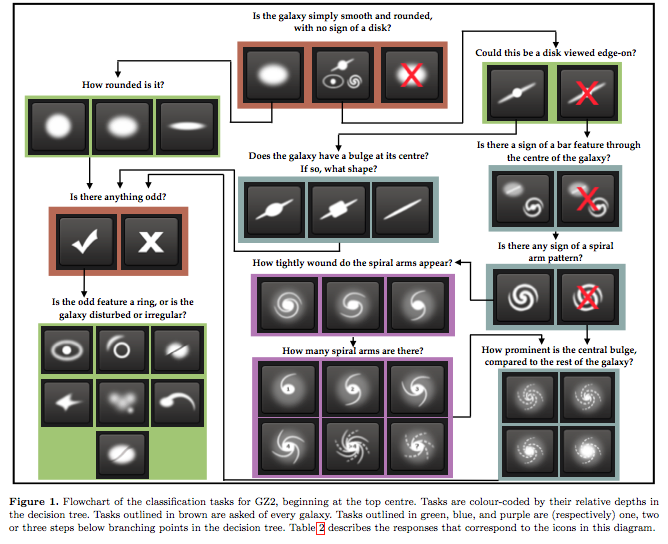
\includegraphics[width=0.48\textwidth, trim=12 60 0 0, clip]{decision_tree.png}
    \caption{Decision tree used to classify galaxies.}
\end{figure}
\FloatBarrier

The galaxy morphology is weighted such that users who tend to agree with the majority are given a higher weight than those who don’t. Thus, the final morphology of the object is a weighted mean of the classifications of all users who analyzed it. As an example, the following is the manual classification results for galaxy id \texttt{100008}: \\

\begin{tabularx}{0.44\textwidth}{ | X | c | c | c | }
       \hline
       \textbf{Galaxy ID} & \textbf{Class 1.1} & \textbf{Class 1.2} & \textbf{Class 1.3} \\
       \hline
       1000008 & 0.383147 & 0.616853 & 0.0 \\
       \hline
\end{tabularx} \\\\

This means that, at the top of the decision tree, 38.31\% of users chose the path that classified galaxy \texttt{100008} into \emph{Class 1.1} for the first question, 61.69\% of users chose the path that classified galaxy \texttt{1000008} into \emph{Class 1.2} for the first question, and 0\% into \emph{Class 1.3}, the last path for the first question. \\

The images below show the most representative images from classes \emph{1.1}, \emph{1.2}, and \emph{1.3} (i.e. the top two images that were classified with the most confidence into those classes by \emph{GalaxyZoo}).

\plottwoimages{../Dataset/105447.jpg}{../Dataset/110858.jpg}{Examples of \emph{Class 1.1} (round galaxies).}
\plottwoimages{../Dataset/100859.jpg}{../Dataset/103950.jpg}{Examples of \emph{Class 1.2} (spiral galaxies).}
\plottwoimages{../Dataset/126783.jpg}{../Dataset/345209.jpg}{Examples of \emph{Class 1.3} (starts/noise).}

From these three classes and their most representative members it can be seen that certain features do seem to vary significantly from class to class. Thus, some feature engineering (ellipsis eccentricity, galaxy radius, and brightness could) could help in the classification process. \\

To match the time requirements of this project and because of the lack of experience dealing with \emph{probability distributions} in a classification problem, we decided to simplify the labels, so that the shape of a galaxy is the one determined by the result of following the highest classification probabilities through the decision tree, so that we finally had a total of 37 possible categories.

\newpage
\section{Classification}
\subsection{Preprocessing}
Since the images show a good amount of noise and artifact, we thought about preprocess the data to get better results. We wanted to feed into the algorithm, only the center galaxy, so we used the method exposed in \cite{cui14}, that allows to remove everything surrounding the center galaxy. As the paper explains:

\begin{quotation}
``\emph{Firstly, for a given galaxy image, we convert the image from \texttt{RGB} color space to gray-scale and use a spatial \emph{Gaussian Smoothing Filter} to remove the noise from the gray-scale image. Secondly, we use \emph{the Otsu’s method} to adaptively find the threshold and segment the original image into a binary image. After that, we fill the holes in the binary image based on morphological operations. Then, we find the biggest connected component located in the center as our target galaxy.}"
\end{quotation}

We applied this method with very good results, as can be seen in the following figures.

\plottwoimages{../Dataset/101325.jpg}{../CleanDataset/101325.jpg}
{Before and after applying the preprocessing step.}
\plottwoimages{../Dataset/102015.jpg}{../CleanDataset/102015.jpg}
{Before and after applying the preprocessing step.}


\subsection{Approach}
Once we have removed parts of the images that may conflict with our approach and extracted only the center galaxy, we obtain the \emph{SIFT} descriptors for each image in the training set. For that purpose, the \emph{VLFeat} implementation of \emph{SIFT} was used \cite{vlfeat}. \\

\plottwoimages{../Images/SIFT example 3 (non-filtered, 50 descriptors, no frames).png}{../Images/SIFT example 3 (non-filtered, 50 descriptors, with frames).png}
{\emph{SIFT} feature descriptors and frames for a \emph{non-clean image} (number of descriptors limited to 50). As can be seen, most the descriptors are taken from the noise instead from the actual galaxy.}

\plottwoimages{../Images/SIFT example 3 (50 descriptors, no frames).png}{../Images/SIFT example 3 (50 descriptors, with frames).png}
{\emph{SIFT} feature descriptors and frames for a \emph{clean image} (number of descriptors limited to 50).}

Then, we quantize the \emph{SIFT} descriptors using \emph{K-means} clustering. The resulting clusters are then stored in a database (a codebook) to be used while quantizing the test samples. The quantification of the \emph{SIFT} descriptors is required to normalize them and make them usable in the classification step. \\

Next, we train the \emph{SVM} using the quantized descriptors from the training data. Once, the \emph{SVM} have been trained (one for each response to every question in the decision tree), we use them to classify the test images. \\

\plottwoimages{../Images/SIFT example 6 (non-filtered, non-limited descriptors, no frames).png}{../Images/SIFT example 6 (non-filtered, non-limited descriptors, with frames).png}
{\emph{SIFT} feature descriptors and frames for a \emph{non-clean image} (non-limited number of descriptors). Again, it can be seen, most the descriptors are taken from the noise instead from the actual galaxy.}

\plottwoimages{../Images/SIFT example 5 (non-limited descriptors, no frames).png}{../Images/SIFT example 5 (non-limited descriptors, with frames).png}
{\emph{SIFT} feature descriptors and frames for a \emph{clean image} (non-limited number of descriptors).}

In order to analyze and compare the effectiveness of our approach, we performed two modifications to our method and then looked at the resulting differences. \\

The first modification we tried was to use \emph{HOG} descriptors instead of \emph{SIFT} descriptors. Again, the \emph{VLFeat} implementation was used \cite{vlfeat}. \emph{HOG} descriptors are represented by a three-dimensional matrix, whose dimensions depend on a parameter, the \emph{cell size}. Thus, for a fixed \emph{cell size}, all the images produce matrices of the same size. As a result, no vector quantification is needed. Then, each \emph{HOG} feature descriptor matrix is transformed into a vector, which we call the feature vector and feed into the \emph{SVM}. \\

% HOG images.
\plottwoimages{../Images/HOG example 2 image (cellSize 4).png}{../Images/HOG example 2 descriptors (cellSize 4).png}
{\emph{HOG} feature descriptors for a \emph{clean image} (\emph{cell size} of 4).}

\plottwoimages{../Images/HOG example 3 image (cellSize 8).png}{../Images/HOG example 3 descriptors (cellSize 8).png}
{\emph{HOG} feature descriptors for a \emph{clean image} (\emph{cell size} of 8).}

The second modification still uses \emph{SIFT} descriptors; however, for every image we only calculate one 128-dimensional \emph{SIFT} descriptor centered and with a given \emph{scale}. Here too, quantification is unnecessary, so we feed this \emph{SIFT} descriptor into the \emph{SVM}. \\

% Single SIFT images.
\plottwoimages{../Images/Single-SIFT example 2 image (scale 5).png}{../Images/Single-SIFT example 2 descriptor (scale 5).png}
{Single-\emph{SIFT} feature descriptor for a \emph{clean image} (\emph{scale} of 5)}

\plottwoimages{../Images/Single-SIFT example 4 image (scale 10).png}{../Images/Single-SIFT example 4 descriptor (scale 10).png}
{Single-\emph{SIFT} feature descriptor for a \emph{clean image} (\emph{scale} of 10)}

%%%%%%%%%%%%%%%%%%%%%%%%%%%%%%%%%%%%%%%%%%%%%%%%%%%%%%%%%%%%%%%%%%
\subsection{Results}
The number of available training images from the dataset is 61,578, while the number of testing images is 79,975. Because obtaining the \emph{SIFT} descriptors of an image is a computationally intensive task, we used only a randomly sampled part of training data and testing date to create both datasets. \\

First, we compared how the three approaches behave in terms of accuracy and execution time depending on the preprocessing of the dataset. In one hand, the clean test data, it is the result of filtering the image to keep only the galaxy while reducing the noise, as explained in the preprocessing section. On the other hand, the test data is the one coming directly from the original dataset.

\begin{figure}[!ht]
    \centering
    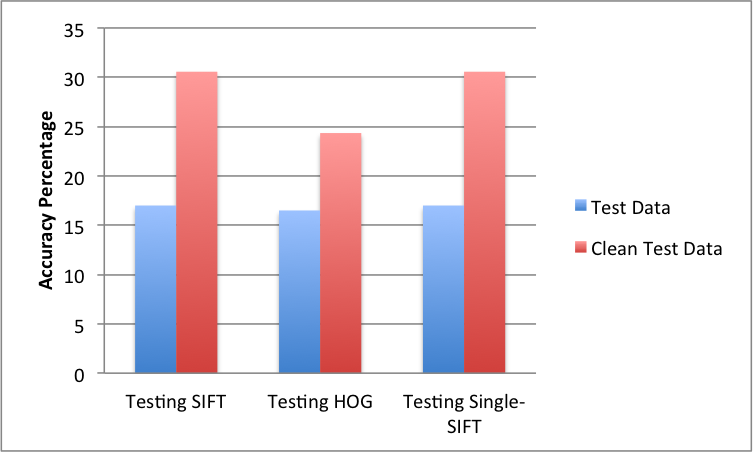
\includegraphics[width=0.48\textwidth, trim=0 0 0 0, clip]{../Images/6_CleanVsReg.png}
    \caption{Comparison of the accuracy obtained depending on the preprocessing of the dataset. [\emph{Results obtained using 500 training images and 200 testing images with 300 clusters and a \emph{lambda} of 1E-05.}].}
\end{figure}
\FloatBarrier

\begin{figure}[!ht]
    \centering
    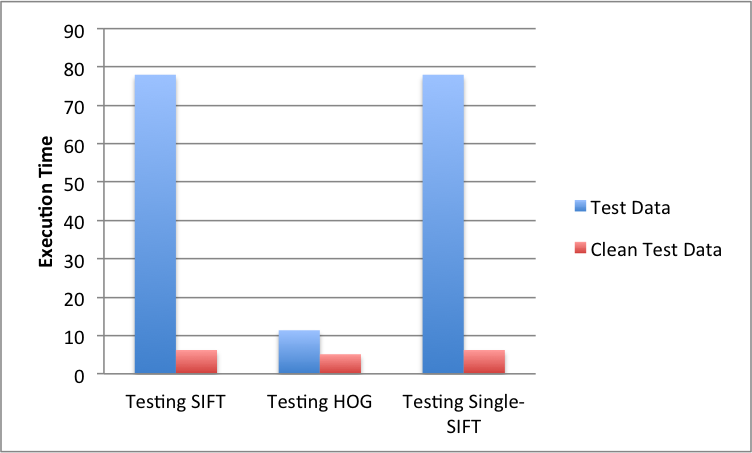
\includegraphics[width=0.48\textwidth, trim=0 0 0 0, clip]{../Images/7_ExecutionTime.png}
    \caption{Comparison of the execution time (in seconds) obtained depending on the preprocessing of the dataset. [\emph{Results obtained using 500 training images and 800 testing images with 200 clusters and a \emph{lambda} of 1E-05.}].}
\end{figure}
\FloatBarrier

As can be seen, in any case, the preprocessed dataset obtains better results both in terms of accuracy and execution time. Therefore, the rest of the results have been gathered using this clean data. \\

Next, we compared how the amount of training data affected the accuracy of the classification of test data. It is clear that it doesn't make a significant change in the accuracy.

\begin{figure}[!ht]
    \centering
    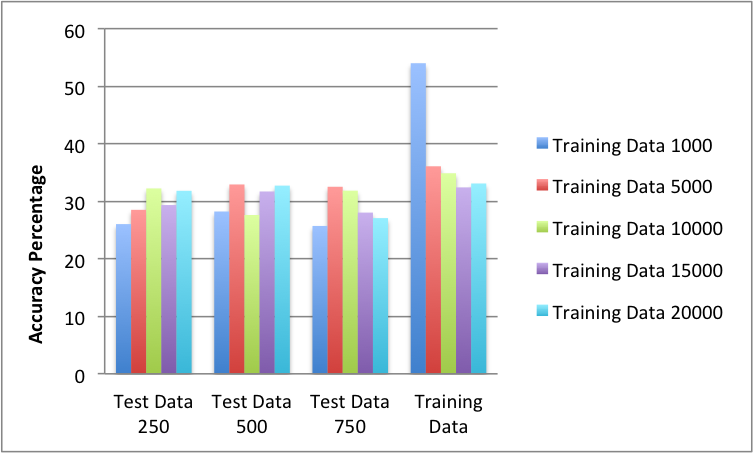
\includegraphics[width=0.48\textwidth, trim=0 0 0 0, clip]{../Images/1_VaryingTrainingData.png}
    \caption{Comparison of how the amount of training data affects the accuracy of classification of test data (\emph{y-axis}). As can be seen, the amount of training data doesn't seem to affect the accuracy obtained. [\emph{Results obtained using 300 clusters and 1E-03 \emph{lambda} for \emph{SVM}}].}
\end{figure}
\FloatBarrier

We also experimented with the \emph{lambda} parameter of the \emph{SVM}, which also determines the number of iterations, and with the number of clusters used in \emph{K-means} (\emph{K} parameter). \\

On one hand, in the case of the training data, it can be seen that as we increased any of them, the accuracy of the results improves. On the other hand, for the test data, a lower \emph{lambda} increases the accuracy till a certain point, probably due to \emph{overfitting} when the value is too low. The number of clusters doesn't seem to have a significant impact on the results.

\begin{figure}[!ht]
    \centering
    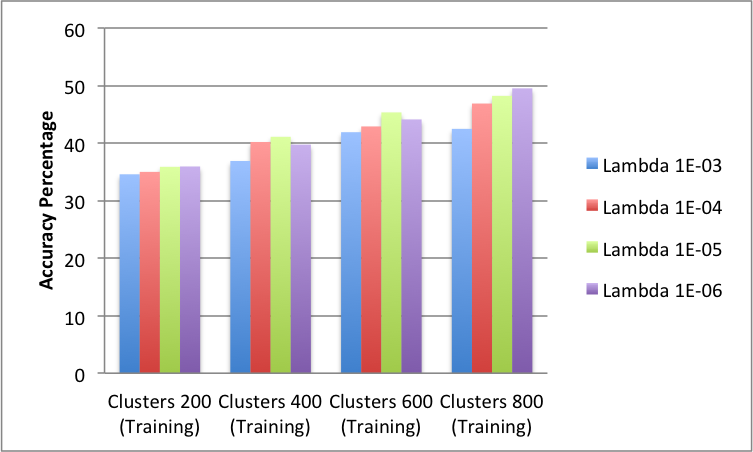
\includegraphics[width=0.48\textwidth, trim=0 0 0 0, clip]{../Images/2_ClustersTraining.png}
    \caption{Comparison of how the variations of the number of clusters and the \emph{lambda} parameter of \emph{SVM} vary the resulting accuracy in the training set. The growing trend seems pretty clear. [\emph{Results obtained using 5,000 training images}].}
\end{figure}
\FloatBarrier

\begin{figure}[!ht]
    \centering
    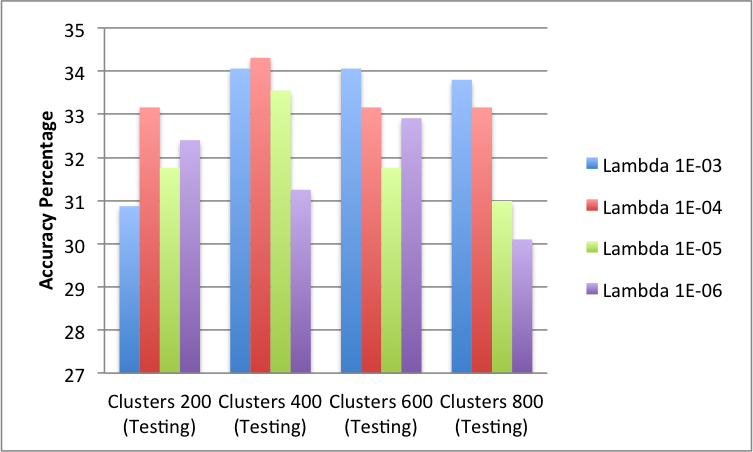
\includegraphics[width=0.48\textwidth, trim=0 0 0 0, clip]{../Images/3_ClustersTesting.png}
    \caption{Comparison of how the variations of the number of clusters and the \emph{lambda} parameter of \emph{SVM} vary the resulting accuracy in the test set. The results show the \emph{overfitting} point of the \emph{SVM} and how the number of clusters doesn't affect significantly. [\emph{Results obtained using 5,000 training images and 800 testing images.}]}
\end{figure}
\FloatBarrier

The effect of changes in the scale of the \emph{single-SIFT} approach is shown in the next figure. The results might suggest that the center part of the galaxies contain more information regarding their morphology than the outside part. This information seems to become undetectable when the \emph{scale} grows up to a certain point, but it appears again when the \emph{scale} matches more or less the size of the galaxy. Clearly, after some point this trend dissapears since the descriptor is much bigger than the galaxy and a lot of noise is added to the feature vector.

\begin{figure}[!ht]
    \centering
    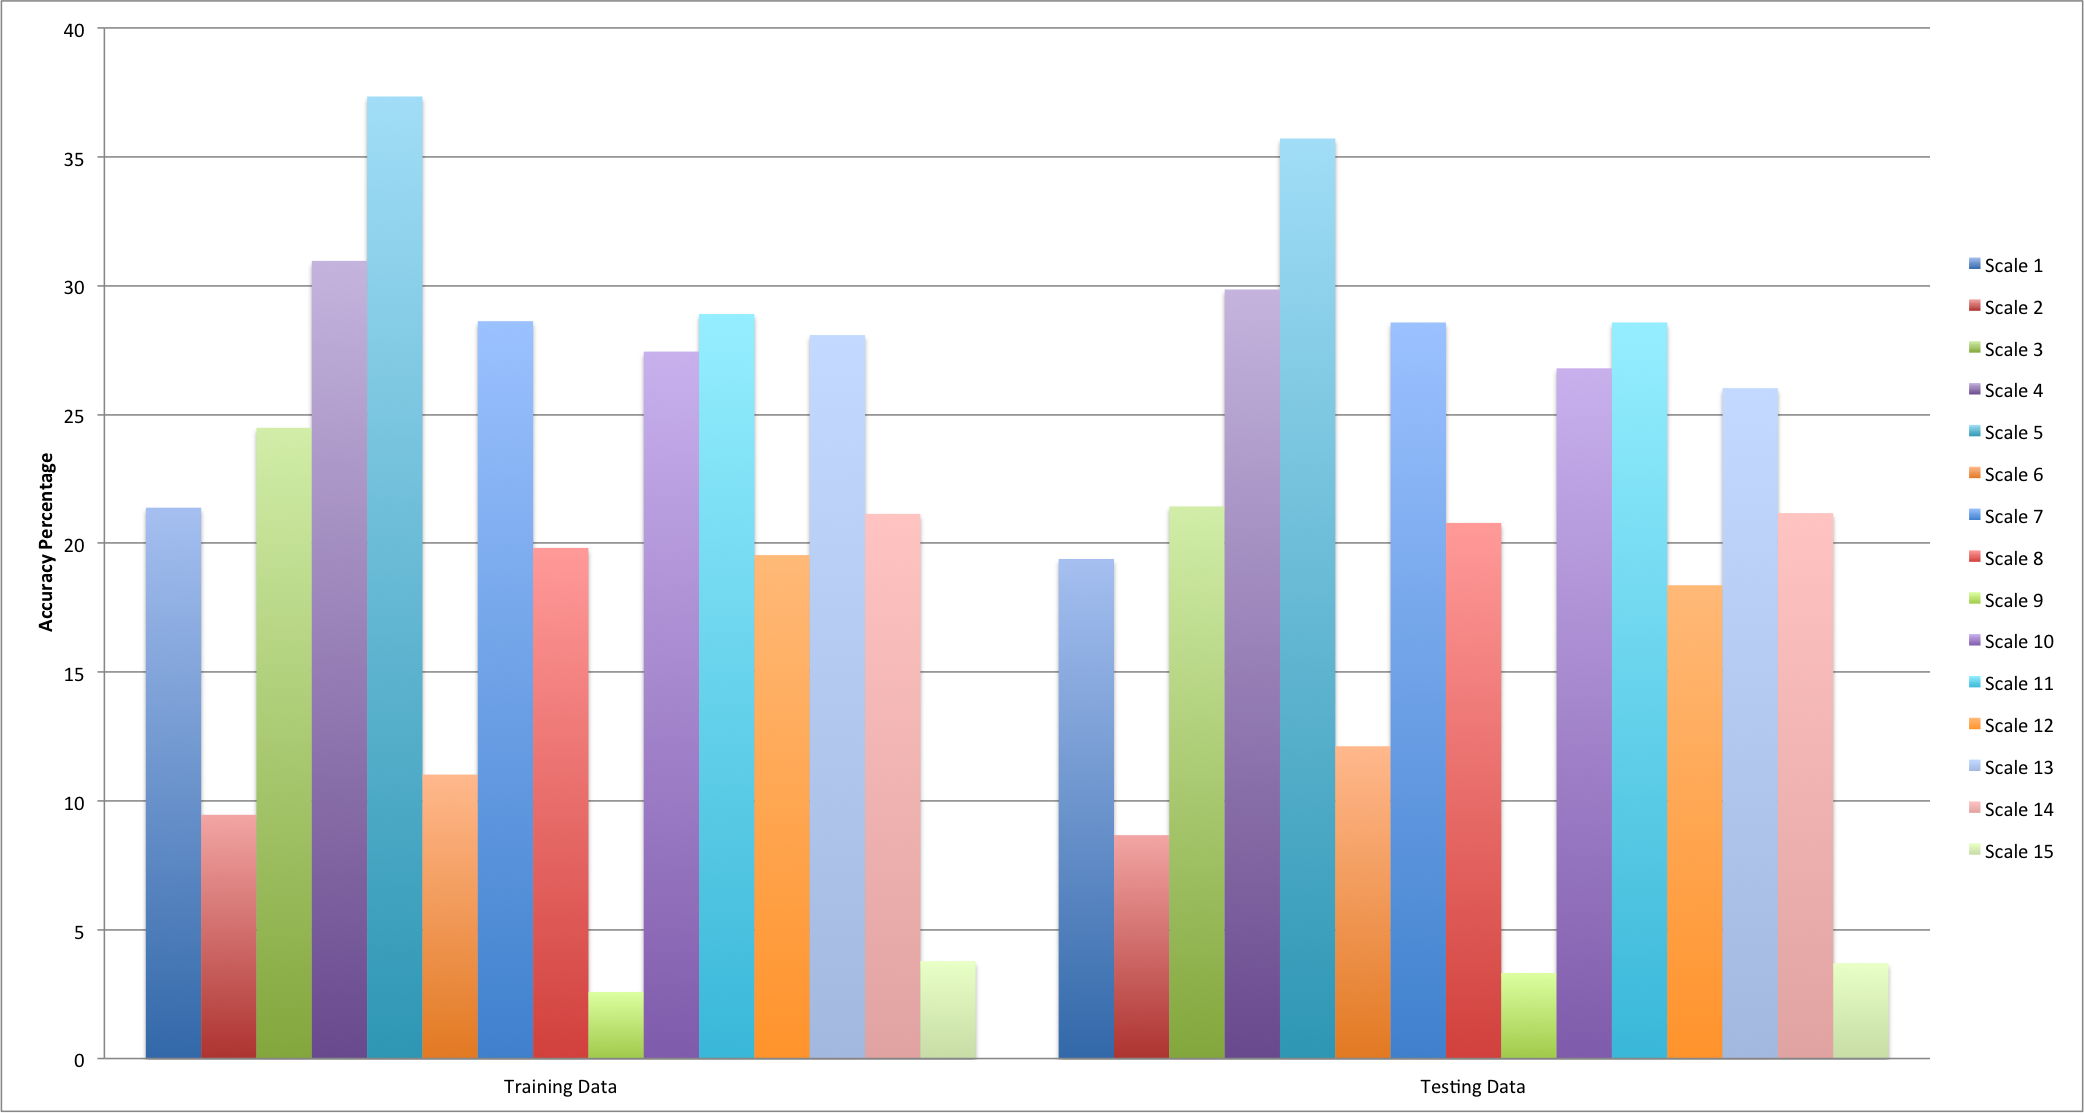
\includegraphics[width=0.48\textwidth, trim=0 0 0 0, clip]{../Images/4_VaryingScaleSingleSIFT.png}
    \caption{Comparison of how the variations of the number of the scale in the \emph{single-SIFT} descriptor approach varies the resulting accuracy in the test set. The results might suggest the distribution of the shape information in the galaxies. [\emph{Results obtained using 5,000 training images and 800 testing images with a \emph{lambda} of 1E-05.}]}
\end{figure}
\FloatBarrier

The same comparison was performed in the case of \emph{HOG} feature descriptors. The results, in this case, show clearly how a different \emph{cell size} used while computing the results doesn't affect them.

\begin{figure}[!ht]
    \centering
    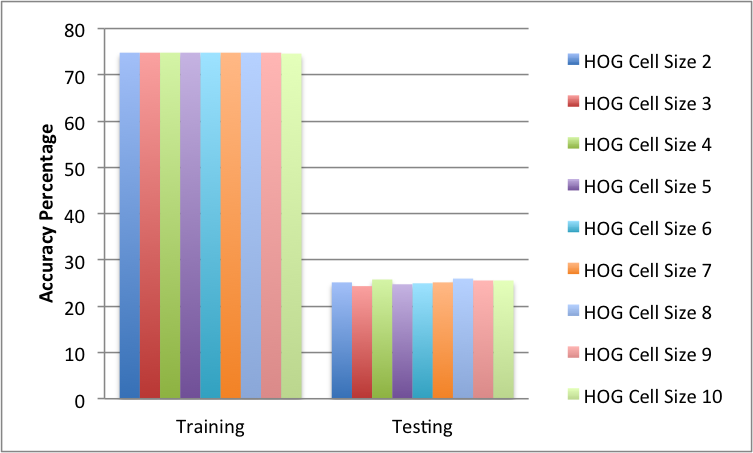
\includegraphics[width=0.48\textwidth, trim=0 0 0 0, clip]{../Images/5_ChangingHOGSize.png}
    \caption{Comparison of how the variations of the \emph{cell size} using \emph{HOG} varies the resulting accuracy in the test set. Clearly, there is no effect. [\emph{Results obtained using 1,000 training images and 500 testing images with a \emph{lambda} of 1E-05.}]}
\end{figure}
\FloatBarrier

\subsection{Conclusions}
In this study, we used a \emph{Machine Learning} algorithm based on \emph{Support Vector Machines} (\emph{SVM}) to perform morphological classifications of images of galaxies taken by modern telescopes. The training and testing input images were manually classified with the help of thousands of volunteers as part of a \emph{GalaxyZoo} project. \\

We considered using many different kinds of descriptors but some of them didn’t fit with our objective. For instance, \emph{GIST} descriptors and \emph{bags-of-features} are often used for whole images. This could be useful if one were trying to program something similar to \emph{Google Goggles}, an app that can detect whether a picture is showing something well-known, like the \emph{Eiffel Tower} or the \emph{Statue of Liberty}. \\

In the end, we opted for \emph{SIFT} descriptors because of their ease of use and highly descriptive capabilities. We quantized the descriptors to normalize them into a uniform size, and we then classified the different galaxy images using the \emph{SVM}. A total of 37 \emph{SVM} were trained, corresponding to each of the 37 possible answers that can be found in the decision tree. We are able to reproduce the human classifications for the galaxies with 30\% accuracy on the testing data. We implemented different variations of our original approach, and we measured and compared how the different parameters affected the accuracy and the time complexity of each modification. In the end, the use quantified \emph{SIFT} descriptors produced the best results. \\

\emph{SIFT} and \emph{HOG} descriptors were the most suited descriptors for our problem. Some limitations to our approach, however, are that \emph{SIFT} descriptors take a long time to extract, and extracting 128 dimensional descriptors for the 61,578 images was computationally intensive, so we decided to randomly sample the datasets given our computational limits. Furthermore, we did not take into account other descriptors which could have increased the accuracy of our classifier. For example, some feature engineering such as extracting the radius of the galaxy and the eccentricity of the ellipse could have helped us distinguish better between round and elliptical galaxies. \\

While 30\% is not a satisfactory result, it is a good starting point. Further research into better feature engineering and preprocessing tool could help increase the accuracy rate. As it is, this approach is not sufficient as a solution to the problem of computationally classifying the morphologies of galaxies. The use of \emph{Convolutional Neural Networks} (\emph{CVN}) seems to be the most promising approach to this problem, as the winner and runner ups of the contest both relied on the power of \emph{CVN} to perform the classification.

\section{Individual contribution}

Our team has had weekly meetings to make sure our project is making progress. When it comes to division of labor, it was decided that it would be determined based on the strengths and interests of each of the members. \\

Ettienne and Andres, through researching different papers on the subject matter, managed to find a way to extract the center galaxies from the image in the process and implemented it. Jose worked on implementing and using \emph{SVM} and \emph{SIFT} descriptors to classify the given galaxies. Ettienne researched other potential methods for feature extraction and for galaxy classification, such as using eigenfaces and neural networks. \\

We collectively read through research papers to discover more approaches. Using \emph{MATLAB} and version control system, \emph{GitHub}, made collaboration very easy to do. We all contributed to the writing of the report by dividing the sections evenly. The poster was also designed in this way. Together, we chose which images to display in the poster and what information seemed the most relevant and explanatory.

% ensure same length columns on last page (might need two sub-sequent latex runs)
\balance

\begin{thebibliography}{9}
\vspace{0.25cm}

\bibitem{kaggle} 
\href{http://www.kaggle.com/c/galaxy-zoo-the-galaxy-challenge}{\emph{Kaggle} \emph{GalaxyZoo} Challenge website.}

\bibitem{vlfeat} 
\href{www.vlfeat.org}{VLFeat website, used for \emph{SIFT} and \emph{HOG} feature extractors.}

\bibitem{lavah08}
Abdalla F. B., Amara A., Capak P., Cypriano E. S., Lahav
O., Rhodes J., 2008, MNRAS, 387, 969

\bibitem{bailer98}
Bailer-Jones C. A. L., Irwin M., von Hippel T., 1998, MN-
RAS, 298, 361

\bibitem{ball04}
Ball N. M., Loveday J., Fukugita M., Nakamura O., Oka-
mura S., Brinkmann J., Brunner R. J., 2004, MNRAS,
348, 1038

\bibitem{banerji08}
Banerji M., Abdalla F. B., Lahav O., Lin H., 2008, MN-
RAS, 386, 1219

\bibitem{cui14}
Cui Y., Xiang Y., Rong K., Feris R., Cao L., 2014, WACV

\bibitem{folkes96}
Folkes S. R., Lahav O., Maddox S. J., 1996, MNRAS, 283,
651

\bibitem{lavah95}
Lahav O., Naim A., Buta R. J., Corwin H. G., de Vaucouleurs G., Dressler A., Huchra J. P., van den Bergh S., Raychaudhury S., Sodre Jr. L., Storrie-Lombardi M. C., 1995, Science, 267, 859

\bibitem{lavah96}
Lahav O., Naim A., Sodr´e Jr. L., Storrie-Lombardi M. C., 1996, MNRAS, 283, 207 

\bibitem{naim95}
Naim A., Lahav O., Sodre Jr. L., Storrie-Lombardi M. C.,
1995, MNRAS, 275, 567

\bibitem{storrie92}
Storrie-Lombardi M. C., Lahav O., Sodre Jr. L., Storrie-
Lombardi L. J., 1992, MNRAS, 259, 8P

\bibitem{vonHippel94}
von Hippel T., Storrie-Lombardi L. J., Storrie-Lombardi
M. C., Irwin M. J., 1994, MNRAS, 269, 97

\end{thebibliography}

%APPENDIX is optional.
% ****************** APPENDIX **************************************
% Example of an appendix; typically would start on a new page
%pagebreak

% \begin{appendix}
% You can use an appendix for optional proofs or details of your evaluation which are not absolutely necessary to the core understanding of your paper. 

% \section{Final Thoughts on Good Layout}
% Please use readable font sizes in the figures and graphs. Avoid tempering with the correct border values, and the spacing (and format) of both text and captions of the PVLDB format (e.g. captions are bold).

% At the end, please check for an overall pleasant layout, e.g. by ensuring a readable and logical positioning of any floating figures and tables. Please also check for any line overflows, which are only allowed in extraordinary circumstances (such as wide formulas or URLs where a line wrap would be counterintuitive).

% Use the \texttt{balance} package together with a \texttt{\char'134 balance} command at the end of your document to ensure that the last page has balanced (i.e. same length) columns.

% \end{appendix}


\end{document}
